% -----------------------------------------------
% Template for ISMIR 2014
% (based on earlier ISMIR templates)
% -----------------------------------------------

\documentclass{article}
\usepackage{ismir2014,amsmath,cite}
\usepackage{graphicx}
\usepackage{amsfonts}
\usepackage{brian}

% Title.
% ------
\title{Hierarchical evaluation of music segment boundary detection}

% Single address
% To use with only one author or several with the same address
% ---------------
%\oneauthor
% {Names should be omitted for double-blind reviewing}
% {Affiliations should be omitted for double-blind reviewing}

% Two addresses
% --------------
\twoauthors
  {First author} {School \\ Department}
  {Second author} {Company \\ Address}

% Three addresses
% --------------
%\threeauthors
  %{First author} {Affiliation1 \\ {\tt author1@ismir.edu}}
  %{Second author} {\bf Retain these fake authors in\\\bf submission to preserve the formatting}
  %{Third author} {Affiliation3 \\ {\tt author3@ismir.edu}}

% Four addresses
% --------------
%\fourauthors
%  {First author} {Affiliation1 \\ {\tt author1@ismir.edu}}
%  {Second author}{Affiliation2 \\ {\tt author2@ismir.edu}}
%  {Third author} {Affiliation3 \\ {\tt author3@ismir.edu}}
%  {Fourth author} {Affiliation4 \\ {\tt author4@ismir.edu}}

\begin{document}
%
\maketitle
%
\begin{abstract}
Structure in music is traditionally analyzed hierarchically: large scale sections at the highest level can be sub-divided and refined down to the short melodic ideas at the motivic level. 
However, typical algorithmic approaches to structural annotation produce flat temporal partitions of a track, which are commonly evaluated against a similarly flat, human-produced
annotation, effectively discarding all notions of structural depth in the annotation.
Recently, collections of hierarchical structure annotations have been published, but at present, no evaluation techniques exist to evaluate against these rich structural annotations.
We propose a method to evaluate structural boundary detection in the context of hierarchical annotation.
The proposed method transforms boundary detection into a ranking problem, and facilitates the comparison of flat and hierarchical annotations.
We demonstrate the proposed method with various synthetic and real world examples. 
\end{abstract}
%
\section{Introduction}\label{sec:introduction}

The analysis of the structure in music has been one of the main areas of interest by musicologists for many years.
Its goal is to identify and categorize the form of a musical piece by investigating the organization of its components, such as sections, phrases, melodies, or recurring motives.
Traditional analyses usually provide multiple levels of annotation (\eg, Schenkerian analysis), which reinforce the general assumption that music is structured hierarchically~\cite{Lerdahl1983a}.
Consequenntly, tree representations are commonly used to both model and analyze hierarchical forms in music~\cite{Lerdahl1983}.

In the music information retrieval literature, \emph{music segmentation} is a task that aims to automatically identify the structure of music~\cite{Paulus2010}.
As opposed to other, more traditional approaches, the segmentation task has generally focused on partitioning a song into non-overlapping segments (or sections).
Nevertheless, it has been shown that even these segments tend to be organized in a hierarchical manner~\cite{Peeters2009}, and even a large dataset of hierarchically-structured human 
annotations is now publicly available~\cite{Smith2011}.
% Still, most existing algorithms only operate at a flat level, likely because (i) this task is already challenging at this level~\cite{Skywalker2014}, and (ii) even if an algorithm could 
% estimate hierarchical segments, no method to evaluate them has been proposed.
However, current evaluation methodologies are defined only for flat segmentations, both in the estimation (algorithm output) and reference human annotation data.  Consequently, the
dimension of \emph{depth} has been practically ignored in the evaluation of music segmentation algorithms.

%This automatic task could facilitate, e.g., the intra-piece navigation, generation of music summaries, or segment-based recommendation systems, especially nowadays when listeners have easy access to large digital music collections.
%Nevertheless, the vast majority of music segmentation algorithms only operate at a flat level instead of following the hierarchical approach that most musicologists follow.

In this work we present the \emph{Segment Hierarchy Agreement Grade} (SHAG), a method to evaluate the accuracy of boundaries in hierarchical segmentations.
The proposed metric works at a frame-level --- similar to the method of Levy and Sandler~\cite{Levy2008}, a score used to evaluate structural annotations --- and it is based on a rank retrieval evaluation where each frame is ranked depending on whether it belongs to the \emph{correct} segment.
The correctness of the segment is evaluated simultaneously across all hierarchical layers, thus resulting in a metric that can both evaluate hierarchical and flat boundaries. (Note
that a flat segmentation is only a specific case of a hierarchical one, where the number of layers is one.)
With SHAG, we facilitate the evaluation of existing flat estimations against hierarchical reference annotations (like those of~\cite{Smith2011}), and encourage new publications on richer hierarchical algorithms.
We demonstrate the behavior of SHAG with multiple synthetic and human examples, and compare the scores with the existing methods when possible.


The rest of the paper is organized as follows: In Section \ref{sec:curr_meth} we review the current evaluation methods of (flat) boundary algorithms. 
Our metric is formally introduced in Section \ref{sec:eval_desc}. 
We provide multiple examples to illustrate the behavior of SHAG in Section \ref{sec:examples}.
Finally, we draw conclusions and discuss future work in Section \ref{sec:conclusions}.

\section{Current Methods}\label{sec:curr_meth}

TODO

\section{Segment Hierarchy Agreement Grade}\label{sec:eval_desc}

\subsection{Music segmentation background}

Let $X \in \mathbb{R}^{d\times n}$ denote a song as represented by a time series of 
feature data, where $d$ denotes the dimension of features, and $n$ denotes the
time duration at some fixed resolution $f_r$ (\eg, 10Hz).
Existing approaches to boundary evaluation pre-suppose a single partitioning into $m$
temporally contiguous regions, so that $X=[X_1|X_2|\cdots|X_m]$.  An estimated
partitioning can then be evaluated by comparing the estimated boundaries between
regions to those in a reference annotation.

Instead, we will suppose that $X$ can be hierarchically decomposed into a tree structure.
In this view, we have segmentations at multiple resolutions or levels of granularity.
The question now is how to evaluate against tree-structured segmentation.

\subsection{Notation}

Let $S \in \mathcal{P}(X)$ denote a temporally contiguous partition of the columns of
$X$.
We will use the subscripts $S_R$ and $S_E$ to denote \emph{reference} and \emph{estimation}, respectively.
$S(i)$ will denote the identifier of the partition containing the $i$th frame (column $X_i$).

Hierarchical segmentations will be denoted by $H$ and follow the subscript conventions
above.  $H(i)$ will denote the most specific segment containing $i$, that is, the
segment containing $i$ at the deepest level in the hierarchy.
$H(i, j)$ will denote the least common ancestor of $H(i)$ and $H(j)$.
We will denote precedence (containment) of segments by $\prec$ and $\preceq$: \eg,
$H(i) \preceq H(i, j)$. 

Note that flat segmentations are a special case of hierarchical segmentations, where there is one node at the root of the hierarchy containing all frames, and then $m$ segments at the next level down which partition $X$.

Restricting to a query frame $q$, $H(q, \cdot)$ induces a partial ranking over the
remaining frames.  Frames contained in $H(q)$ are considered maximally relevant,
followed by those in $H(q)$'s immediate ancestor, and so on.
This observation will be the key to our evaluation, as it provides a connection
between hierarchical time-series decompositions and ranking evaluation.


\subsection{Reduction to ranking}


We can reduce segmentation evaluation to a ranking evaluation problem as follows.
Let $q$ denote an arbitrary frame, and let $i$ and $j$ denote any two frames such that $S_R(q) = S_R(i)$ and $S_R(q) \neq S_R(j)$.
In this case, $i$ may be considered \emph{relevant} for $q$, and $j$ is considered \emph{irrelevant} for $q$.
This leads to a straightforward reduction to bipartite ranking.

Assuming that both $S_E$ and $S_R$ have $n$ frames, we can formally describe a frame
recall metric:
\begin{equation}
f(q ; S_E) \defeq 
\sum_{\substack{i \in S_R(q)\\ j \notin S_R(q)}}
\frac{\ind{S_E(q) = S_E(i) \neq S_E(j) }}{|S_R(q)|\cdot (n -
|S_R(q)|)}.\label{flatrecall}
\end{equation}
That is, the score for frame $q$ is the fraction of pairs $(i, j)$ for which $S_E$
agrees with $S_R$ with respect to $q$ (\ie, membership in the segment).

Averaging over all frames $q$ yields an average frame recall score:
\begin{equation}
\rho(S_E) \defeq \frac{1}{n} \sum_q f(q ; S_E).\label{avgrecall}
\end{equation}
% TODO:   2014-05-05 00:38:15 by Brian McFee <brm2132@columbia.edu>
% talk about why we don't need to consider precision here
% predictions are mutually exclusive
% the usual way to cheat at recall is to make too many predictions..
% but to do that for q1, you'd have to make fewer predictions for q2,
\nocite{levy2008structural}


\subsection{Partial Ranking}

\Cref{flatrecall} is defined in terms of segment membership (in)equalities, but 
we can equivalently express the function using strict precedences in a (flat)
segment hierarchy.
Rather than compare $i$ and $j$ where $S(q) = S(i) \neq S(j)$, we can express this as $H(q, i) \prec H(q, j)$.
That is, $q$ and $i$ merge before $q$ and $j$:
\begin{equation}
g(q ; H_E) \defeq \sum_{\substack{(i, j)\\ H_R(q, i) \prec H_R(q, j)}}
\frac{\ind{H_E(q, i) \prec H_E(q, j)}}{Z_q},\label{hierrecall}
\end{equation}
where $Z_q$ is a normalization term that counts the number of terms in the summation.

Just as in \cref{flatrecall}, $g$ can be viewed as a classification accuracy of
correctly predicting pairs $(i, j)$ as positive ($q$ and $i$ merge first) or negative
($q$ and $j$ merge first).  The case where $H(q, i) = H(q, j)$ is precluded by the
strict precedence operator in the summation.

\Cref{hierrecall} can be alternately be viewed as a generalized area under the curve
(AUC) over the partial ranking induced by the hierarchical segmentation, where the
prediction threshold being varied is the depth within the estimated hierarchy $H_E$.
% Note that the precedence comparisons here are strict, so we never compare two $i$ and $j$ that merge simultaneously with $q$.
Aggregating over all frames $q$, we get the following average recall metric, which we
term the Structural Congruency Index (SCI):
\begin{equation}
SCI(H_E) \defeq \frac{1}{n} \sum_q g(q ; S_E)
\end{equation}

Note this loss is equivalent to that evaluated by for subjective artist similarity~\cite{mcfee2011}.
The difference here is that the reference rankings are induced from ordinal data, and not subject to consistency errors.

\subsection{Windowing in Time}

The calculation of SCI can be expensive ($\Oh\left(n^3\right)$ using a straightforward 
implementation).
The score also varies with $n$, so comparisons between tracks of differing length can
be probematic.  For extreme values of $n$, \cref{hierrecall} may be dominated by pairs
obviously irrelevant comparison points $j$ which lie far from $q$ in time.

Therefore, we propose to use a time window of $w$ seconds in order to both simplify the 
calculation of the metric and normalize its dynamic range.
We restrict the number of frames to consider to $m = \lceil w \cdot f_r \rceil$.
Adding this windowing property to the SIC equations yields:
\begin{equation}
  g(q, m ; H_E) \defeq \sum_{\substack{
  m_s \leq i,j \leq m_e \\ 
  H_R(q, i) \prec H_R(q, j) }} \frac{\ind{H_E(q, i) \prec H_E(q,
  j)}}{Z_q(m)},\label{windowrecall}
\end{equation}
\begin{equation}
SIC(H_E,m) \defeq \frac{1}{n} \sum_q g(q,m ; S_E),
\end{equation}
where $m_s = \min\{0,q-m/2\}$ and $m_e = \max\{q+m/2,n\}$ are the start and ending, respectively, of the current window in frame indices.

FIXME: Move this next part down to 3.1

Small windows (\eg, $w \leq 3$) only capture the local changes, 
losing precision since most of the segments will be more than this small window.
We want a window that is long enough to capture the boundaries of the current segments, and that is the same for all tracks in order to be able to easily compare results within a reasonable dynamic range.
In the task of music segmentation, most of the segments will be less than 45 seconds (30?).

\subsection{Transitivity}

Just as \cref{hierrecall} can be dominated by long-range interactions in the absence
of windowing, deep hierarchies can also pose a problem.  To see this, consider the 
sequence $H_R(q, i) \prec H_R(q, j) \prec H_R(q, k)$.  Due to the transitive
containment structure of $H_R$, we have $i \in H_R(q, i) \subseteq H_R(q, j)$.
Since the summation in \cref{hierrecall} ranges over all precedence comparisons, the
pair $(i, k)$ appears twice in the summation.  

To counteract this effect, the summation can be restricted to only range over direct
precedence relations.  In practice, this is accomplished by only comparing frames from
successive levels in the hierarchy.  As a result, redundant comparisons are
eliminated, and the dynamic range of $g$ is increased.

\subsection{Choosing a Time Window}

TODO

\section{Examples}\label{sec:examples}

In this section we discuss the behavior of SHAG by showing various synthetic examples, and compare them against other existing methods when possible.
Two different versions of each metric are used to evaluate these examples: Estimated against Reference boundaries (E2R), and the Reference boundaries against the Estimated ones (R2E).
These results will help us illustrate the variation of the scores when swapping the references with the estimations, which, in the case of SHAG, has a significant impact.
Moreover, we show various window times $w$ to better capture the behavior of our proposed metric.
We subdivide this section based on the type of annotations to be evaluated.

\subsection{Flat vs Flat}

To start with, we compare two flat boundary annotations (i.e. one-layer), and see how SHAG behaves compared to the standard hit rate measure at 3 seconds and the median deviations.
The synthesized flat boundaries are displayed in Figure \ref{fig:flat-flat}, and they aim to capture the situation where an algorithm only estimates --without any time deviations-- a subset of all the reference boundaries.

\begin{figure}
  \centering
  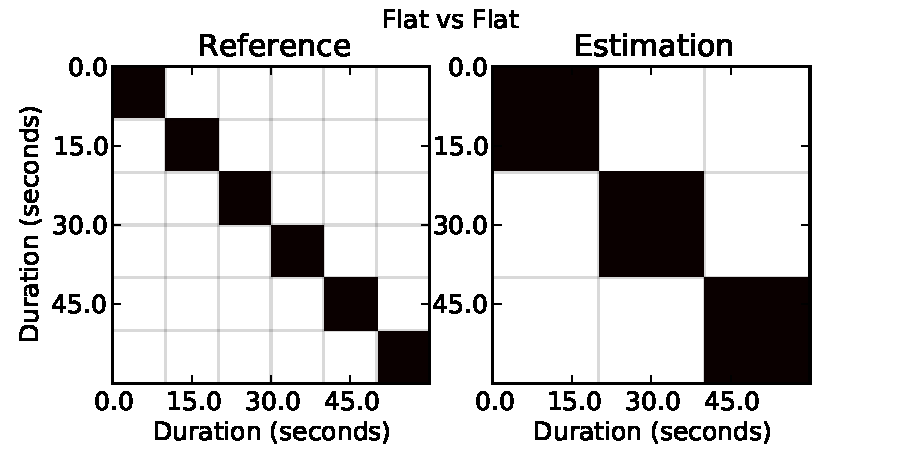
\includegraphics[width=0.47\textwidth]{plots/flat-flat.pdf}
  \caption{Visual representation of flat boundaries.}
  \label{fig:flat-flat}
\end{figure}%

Since we are evaluating flat annotations, we can compute the standard metrics as well. The hit rate scores (top right part of Table \ref{tab:flat-flat}) obtain a precision of 100\% for the E2R type, since all the estimated boundaries are also in the reference.
On the other hand, only four out of seven boundaries were retrieved, so the recall value is 40\%, leaving the F-measure at 57.14\%.
When swapping the reference with the estimation (i.e. R2E type), the F-measure remains the same, but the precision and recall switch values as expected.
The median deviations, displayed on the bottom right of Table \ref{tab:flat-flat}, are always 0 seconds (i.e. highest possible score) since we did not add any fluctuation in the boundaries.
It becomes apparent how the medians can not always be reliable, since two sets of boundaries can be quite different while still obtaining the best results for this metric.

\begin{table}
 \begin{center}
   \begin{tabular}{|c|c|c||c|c|c|c|}
  \hline
  \multicolumn{3}{|c||}{\textbf{SHAG}} & \multicolumn{4}{c|}{\textbf{Hit Rate (trimmed)}} \\
  \hline
  $w$ & $H_u$   & $H_o$ & Type & $F$     & $P$     & $R$ \\
  \hline
  0.5       & 40.0   & 100   & E2R & 57.14  & 100 & 40.0 \\
  3         & 40.0   & 100   & R2E & 57.14  & 40.0 & 100  \\
  \cline{4-7}
  15        & 39.39  & 52.77 & \multicolumn{4}{c|}{\textbf{Median Deviations}}   \\
  \cline{4-7}
  30        & 69.49  & 49.75 & \multicolumn{2}{c|}{E2R} & \multicolumn{2}{c|}{R2E} \\
  \cline{4-7}
  $\infty$  & 80.0   & 49.75 & \multicolumn{2}{c|}{0} & \multicolumn{2}{c|}{0}  \\
  \hline
 \end{tabular}
\end{center}
  \caption{Flat vs flat scores}
  \label{tab:flat-flat}
\end{table}

E2R == Undersegmented
R2E == Oversegmented

The SHAG scores for the flat annotations are shown on the left side of Table \ref{tab:flat-flat}.
For the shorter time windows of 0.5 and 3 seconds 

TODO: Trimming boundaries recall hit-rate work a bit like short window times of the E2R of SHAG.


\subsection{Hierarchical vs Flat}

\begin{figure}
  \centering
  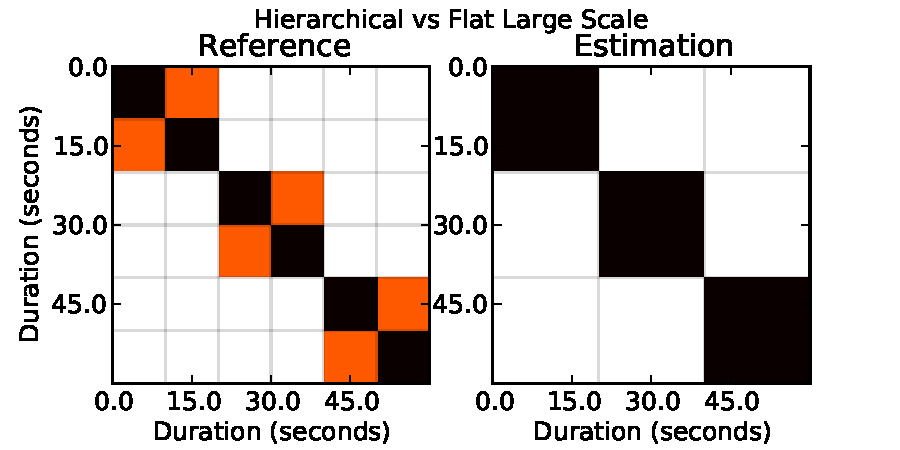
\includegraphics[width=0.47\textwidth]{plots/hier-flatlarge.pdf}
  \caption{TODO}
  \label{fig:hier-flatlarge}
\end{figure}%

\begin{table}
 \begin{center}
   \begin{tabular}{|c|c|c|}
  \hline
  \multicolumn{3}{|c|}{\textbf{SHAG}} \\
  \hline
  $w$       & $H_u$    & $H_o$      \\
  \hline
  0.5       & 0         & 100      \\     
  3         & 0         & 100      \\
  15        & 37.21     & 100    \\
  30        & 69.66     & 100    \\
  $\infty$  & 80.16     & 100    \\
  \hline
 \end{tabular}
\end{center}
  \caption{Hierarchical vs Flat Large Scale}
  \label{tab:hier-flatlarge}
\end{table}

\begin{figure}
  \centering
  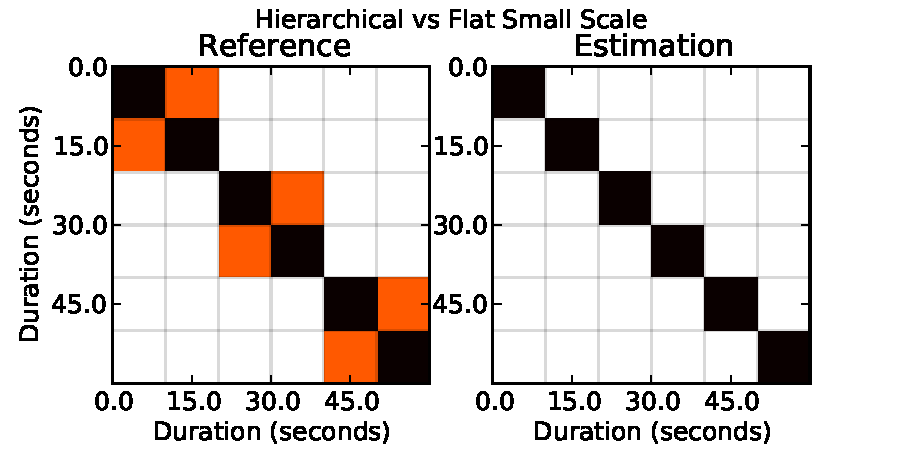
\includegraphics[width=0.47\textwidth]{plots/hier-flatsmall.pdf}
  \caption{TODO}
  \label{fig:hier-flatsmall}
\end{figure}%

\begin{table}
 \begin{center}
   \begin{tabular}{|c|c|c|}
  \hline
  \multicolumn{3}{|c|}{\textbf{SHAG}} \\
  \hline
  $w$       & $H_u$    & $H_o$      \\
  \hline
  0.5       & 100       & 100      \\     
  3         & 100       & 100      \\
  15        & 62.79     & 100    \\
  30        & 30.34     & 100    \\
  $\infty$  & 19.84     & 100    \\
  \hline
 \end{tabular}
\end{center}
  \caption{Hierarchical vs Flat Small Scale}
  \label{tab:hier-flatsmall}
\end{table}
ok

\subsection{Hierarchical vs Hierarchical}

\begin{figure}
  \centering
  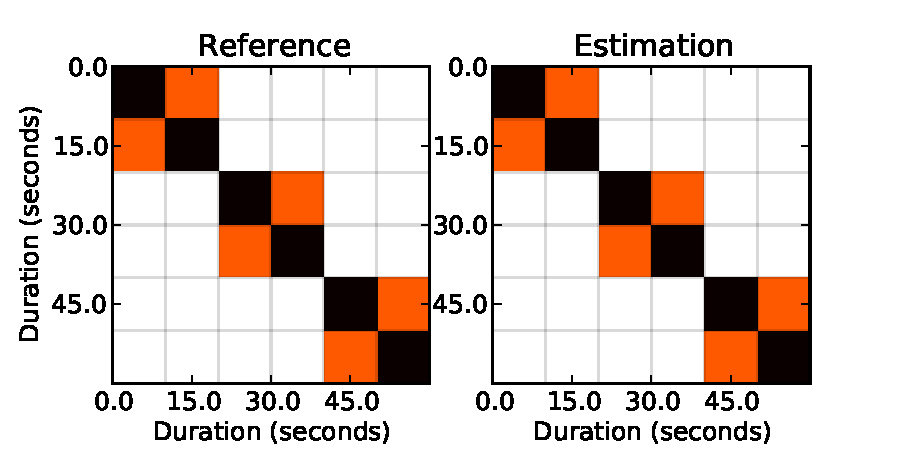
\includegraphics[width=0.47\textwidth]{plots/hier-hier.pdf}
  \caption{TODO}
  \label{fig:hier-hier}
\end{figure}%

\begin{table}
 \begin{center}
   \begin{tabular}{|c|c|c|}
  \hline
  \multicolumn{3}{|c|}{\textbf{SHAG}} \\
  \hline
  $w$       & $H_u$    & $H_o$      \\
  \hline
  any       & 100       & 100      \\     
  \hline
 \end{tabular}
\end{center}
  \caption{Hierarchical vs Hierarchical}
  \label{tab:hier-hier}
\end{table}

\begin{figure}
  \centering
  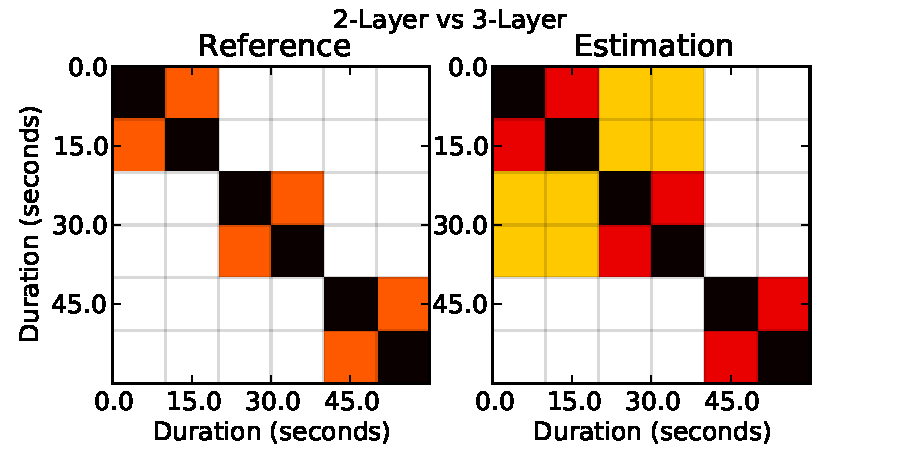
\includegraphics[width=0.47\textwidth]{plots/hier-hiercomp.pdf}
  \caption{TODO}
  \label{fig:hier-hiercomp}
\end{figure}%

\begin{table}
 \begin{center}
   \begin{tabular}{|c|c|c|}
  \hline
  \multicolumn{3}{|c|}{\textbf{SHAG}} \\
  \hline
  $w$       & $H_u$       & $H_o$      \\
  \hline
  0.5       & 100       & 100      \\     
  3         & 100       & 100      \\
  15        & 100       & 98.32    \\
  30        & 100       & 78.81    \\
  $\infty$  & 100       & 61.85    \\
  \hline
 \end{tabular}
\end{center}
  \caption{2-Layer Hierarchical vs 3-Layer Hierarchical}
  \label{tab:hier-hiercomp}
\end{table}


\section{Evaluating Automatic Algorithm}

Olda\cite{McFee2014} with SALAMI.


%\begin{table}
 %\begin{center}
 %\begin{tabular}{|l|l|}
  %\hline
  %String value & Numeric value \\
  %\hline
  %Hello ISMIR  & 2014 \\
  %\hline
 %\end{tabular}
%\end{center}
 %\caption{Table captions should be placed below the table.}
 %\label{tab:example}
%\end{table}

%\begin{figure}
 %\centerline{\framebox{
 %\includegraphics[width=\columnwidth]{figure.png}}}
 %\caption{Figure captions should be placed below the figure.}
 %\label{fig:example}
%\end{figure}

\section{Conclusions}\label{sec:conclusions}

Our method will save us all.

\bibliography{refs}

%\bibliography{ismir2014template}

\end{document}
